

\colorlet{outlinecolor}{orange}

\colorlet{headercolor}{outlinecolor}
\colorlet{rowcolor1}{outlinecolor!70}
\colorlet{rowcolor2}{outlinecolor!50}

\begin{tikzpicture}
	\node [mybox, fill=boxcolor, draw=outlinecolor] (box){%
		\begin{minipage}{0.3\textwidth}
			\vspace{0.1cm}
			\textcolor{outlinecolor}{A repository} is a collection of version controlled files that are kept together. This includes \textbf{(a)} all the files related to a specific project/application, \textbf{(b)} the history of changes, and \textbf{(c)} any special configurations. \\
			
			\vspace{-1mm}
			\underline{Git states}: Git has three \textbf{local} states.
			\begin{enumerate}
				\item The \textcolor{outlinecolor}{working directory state} holds all the project or application files. These files may or may not be managed by Git, but Git is aware of them.
				\item The \textcolor{outlinecolor}{staging area state} or \textcolor{outlinecolor}{Git index state} is holding area for the queue of changes to be included in your next commit.
				\item The \textcolor{outlinecolor}{local Git repository state}  is a hidden folder called \inlinebash{.git}, which contains your entire local commit history.
			\end{enumerate}
			Git also has a \textcolor{outlinecolor}{remote (repository) state}, which is just another repository with its own three internal states. A specific Git command is used to move files between these states. i.e., \\
			
			\begin{minipage}{\textwidth}
				\centering
%				\vspace{-2mm}
				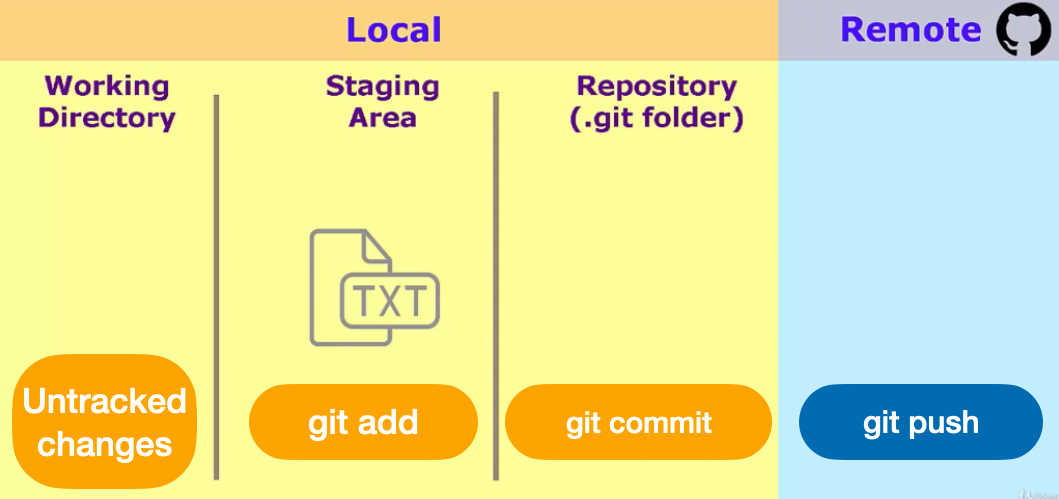
\includegraphics[width=0.5\textwidth]{images/git_stages.png}
				\vspace{-2mm}
				\captionof{figure}{Git states and associated commands. \href{https://www.udemy.com/course/git-complete/}{ \faLink{}  Source}}
			\end{minipage}
			
		\vspace{-3mm}
		\end{minipage}
	};
	\node[fancytitle, right=10pt, fill=outlinecolor, text=background, draw=outlinecolor, rounded corners] at (box.north west) {Git Theory};
\end{tikzpicture}
\begin{tikzpicture}
	\node [mybox, fill=boxcolor, draw=outlinecolor] (box){%
		\begin{minipage}{0.3\textwidth}
			\vspace{0.1cm}
			\underline{Tracking}: A \textcolor{outlinecolor}{tracked file}  is any file that Git is aware of and is actively tracking. In other words, any files that aren't new.
			

		\begin{center}
			\textcolor{background}{
				    \begin{tabularx}{\textwidth}{>{\columncolor{rowcolor1}}X|>{\columncolor{rowcolor2}}p{5cm}}
					\arrayrulecolor{boxcolor} % Table line color
					\rowcolor{headercolor} % Header row color
						\multicolumn{1}{c|}{\centering \textbf{Git Command}} & \multicolumn{1}{c}{\centering \textbf{Description}} \\ % Center the header text
					\hline % Add a horizontal line below the header row
					\rowcolor{rowcolor1} \tablebash{git ls-files} & Returns the list of files tracked by Git \\
					\rowcolor{rowcolor2} % Color of the second row
					\tablebash{git commit -am "commit message"} & Simultaneously add and commit a tracked file \\
					\rowcolor{rowcolor1} \tablebash{git add .} & Recursively add untracked files from current filepath location \\
				\end{tabularx}
			}
		\end{center}
		
		
%		\begin{center}
%			\textcolor{background}{
%				\begin{tabularx}{\textwidth}{>{\columncolor{rowcolor1}}X|>{\columncolor{rowcolor2}}p{5.5cm}}
%					\arrayrulecolor{boxcolor}
%					\rowcolor{headercolor}
%					
%					\hline
%					\rowcolor{rowcolor1} \tablebash{hi} & \multic
%					
			
		\end{minipage}
	};
	\node[fancytitle, right=10pt, fill=outlinecolor, text=background, draw=outlinecolor, rounded corners] at (box.north west) {Git Theory (2)};
\end{tikzpicture}
